\documentclass[12pt,fleqn]{article}\usepackage{../../common}
\begin{document}
Sıvılar - 2

Doğu-Batı yönü E,W ile Kuzey-Güney yönü N,S ile Yukarı-Aşağı yönü T,S
ile belirtilecek. 

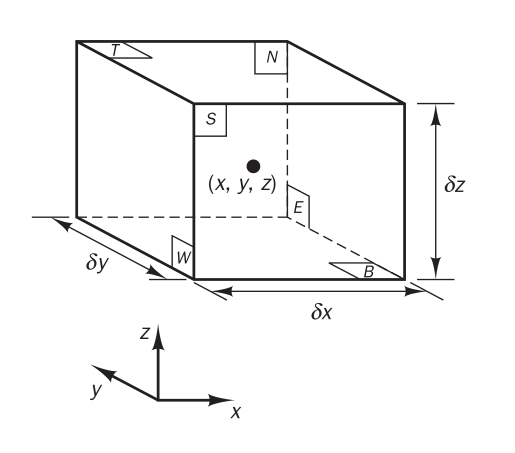
\includegraphics[width=15em]{phy_030_fluid2_03.png}

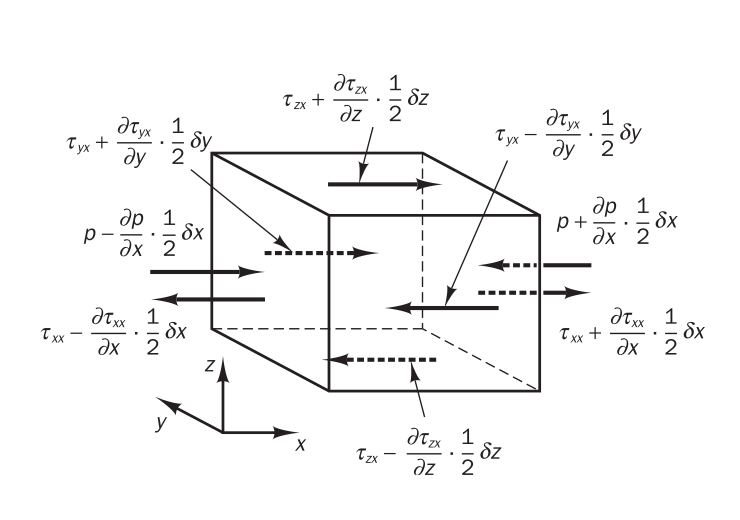
\includegraphics[width=20em]{phy_030_fluid2_01.png}

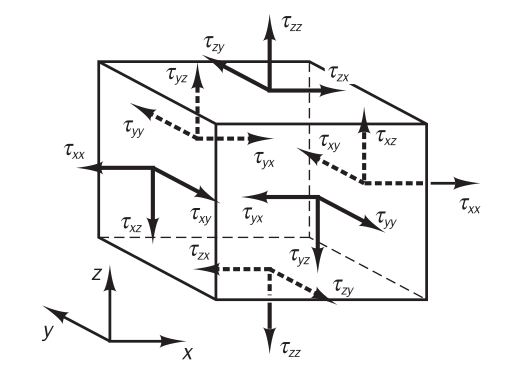
\includegraphics[width=15em]{phy_030_fluid2_02.png}




$$
\left[
  \left( p - \frac{\partial p}{\partial x} \frac{1}{2} \delta x \right) -
  \left( \tau_{xx} - \frac{\partial \tau_{xx}}{\partial x} \frac{1}{2} \delta x \right) 
\right]
  \delta y \delta z  +
\left[
  -\left( p + \frac{\partial p}{\partial x} \frac{1}{2} \delta x \right) +
  \left( \tau_{xx} + \frac{\partial \tau_{xx}}{\partial x} \frac{1}{2} \delta x \right) 
  \delta y \delta z  +  
\right]
$$

$$
= \left(
-\frac{\partial p}{\partial x} + \frac{\partial \tau_{xx}}{\partial x}
\right)
\delta x \delta y \delta z
$$





Kaynaklar

[1] Versteeg, {\em An Introduction to CFD}

\end{document}
